\documentclass[a4paper]{article}

\input{style/ch_xelatex.tex}
\input{style/scala.tex}

%代码段设置
\lstset{numbers=left,
basicstyle=\scriptsize,
numberstyle=\scriptsize,
keywordstyle=\color{blue!70},
commentstyle=\color{red!50!green!50!blue!50},
frame=single, rulesepcolor=\color{red!20!green!20!blue!20},
escapeinside=``
}

\graphicspath{ {../report/pic/} }
\usepackage{ctex}
\usepackage{color,framed}%文本框
\usepackage{listings}
\usepackage{caption}
\usepackage{amssymb}
\usepackage{enumerate}
\usepackage{xcolor}
\usepackage{bm} 
\usepackage{lastpage}%获得总页数
\usepackage{fancyhdr}
\usepackage{tabularx}  
\usepackage{geometry}
\usepackage{listings}
\usepackage{graphics}
\usepackage{subfigure}
\usepackage{float}
\usepackage{pdfpages}
\usepackage{pgfplots}
\pgfplotsset{width=10cm,compat=1.9}
\usepackage{multirow}
\usepackage{footnote}
\usepackage{booktabs}
\usepackage{array}

% 设置字体大小和行间距为原来的 90%
\renewcommand{\baselinestretch}{0.9}

%-----------------------伪代码------------------
\usepackage{algorithm}  
\usepackage{algorithmicx}  
\usepackage{algpseudocode}  
\floatname{algorithm}{Algorithm}  
\renewcommand{\algorithmicrequire}{\textbf{Input:}}  
\renewcommand{\algorithmicensure}{\textbf{Output:}} 
\usepackage{lipsum}  
\makeatletter
\newenvironment{breakablealgorithm}
  {% \begin{breakablealgorithm}
  \begin{center}
     \refstepcounter{algorithm}% New algorithm
     \hrule height.8pt depth0pt \kern2pt% \@fs@pre for \@fs@ruled
     \renewcommand{\caption}[2][\relax]{% Make a new \caption
      {\raggedright\textbf{\ALG@name~\thealgorithm} ##2\par}%
      \ifx\relax##1\relax % #1 is \relax
         \addcontentsline{loa}{algorithm}{\protect\numberline{\thealgorithm}##2}%
      \else % #1 is not \relax
         \addcontentsline{loa}{algorithm}{\protect\numberline{\thealgorithm}##1}%
      \fi
      \kern2pt\hrule\kern2pt
     }
  }{% \end{breakablealgorithm}
     \kern2pt\hrule\relax% \@fs@post for \@fs@ruled
  \end{center}
  }
\makeatother
%------------------------代码-------------------
\usepackage{xcolor} 
\usepackage{listings} 
\lstset{ 
breaklines,%自动换行
basicstyle=\scriptsize,
escapeinside=``,
keywordstyle=\color{ blue!70} \bfseries,
commentstyle=\color{red!50!green!50!blue!50},% 
stringstyle=\ttfamily,% 
extendedchars=false,% 
linewidth=\textwidth,% 
numbers=left,% 
numberstyle=\scriptsize \color{blue!50},% 
frame=trbl% 
rulesepcolor= \color{ red!20!green!20!blue!20} 
}

%-------------------------页面边距--------------
\geometry{a4paper,left=2.3cm,right=2.3cm,top=2.7cm,bottom=2.7cm}
%-------------------------页眉页脚--------------
\usepackage{fancyhdr}
\pagestyle{fancy}
% \chead{}
\rhead{\kaishu 并行程序设计实验报告}%加粗\bfseries 
\lfoot{}
\cfoot{\thepage}
\rfoot{}
\renewcommand{\headrulewidth}{0.1pt}  
\renewcommand{\footrulewidth}{0pt}%去掉横线
\newcommand{\HRule}{\rule{\linewidth}{0.5mm}}%标题横线
\newcommand{\HRulegrossa}{\rule{\linewidth}{1.2mm}}
\setlength{\textfloatsep}{10mm}%设置图片的前后间距
%--------------------文档内容--------------------

\begin{document}
\renewcommand{\contentsname}{目\ 录}
\renewcommand{\appendixname}{附录}
\renewcommand{\appendixpagename}{附录}
\renewcommand{\refname}{参考文献} 
\renewcommand{\figurename}{图}
\renewcommand{\tablename}{表}
\renewcommand{\today}{\number\year 年 \number\month 月 \number\day 日}

% 设置中文标题序号格式
\renewcommand{\thesection}{\chinese{section}}
\renewcommand{\thesubsection}{（\chinese{subsection}）}
\renewcommand{\thesubsubsection}{\arabic{subsubsection}}

% 删除图表编号并设置字体大小为原来的 60%
\captionsetup[figure]{labelformat=empty, font=scriptsize}
\captionsetup[table]{labelformat=empty, font=scriptsize}

%-------------------------封面----------------
\begin{titlepage}
    \begin{center}
    
\includegraphics[width=0.8\textwidth]{NKU.png}\\[1cm]
    \vspace{20mm}
		\textbf{\huge\textbf{\kaishu{计算机学院}}}\\[0.5cm]
		\textbf{\huge{\kaishu{并行程序设计期末报告}}}\\[2.3cm]
		\textbf{\Huge\textbf{\kaishu{CUP 架构编程实验}}}

		\vspace{\fill}
    
    % \textbf{\Large \textbf{并行程序设计期末实验报告}}\\[0.8cm]
    % \HRule \\[0.9cm]
    % \HRule \\[2.0cm]
    \centering
    \textsc{\LARGE \kaishu{姓名\ :\ 刘宇泽}}\\[0.5cm]
    \textsc{\LARGE \kaishu{学号\ :\ 2411334}}\\[0.5cm]
    \textsc{\LARGE \kaishu{专业\ :\ 计算机科学与技术}}\\[0.5cm]
    
    \vfill
    {\Large \today}
    \end{center}
\end{titlepage}

\renewcommand {\thefigure}{\thesection{}.\arabic{figure}}%图片按章标号
\renewcommand{\figurename}{图}
\renewcommand{\contentsname}{目录}  
\cfoot{\thepage\ of \pageref{LastPage}}%当前页 of 总页数


% 生成目录
\clearpage
\begingroup
\renewcommand{\baselinestretch}{1.6}
\tableofcontents
\endgroup
\newpage

%--------------------------摘要--------------------------------
\section{摘要}
本实验围绕现代 CPU 架构的两个核心性能优化方向展开：一是通过优化访存模式提升 Cache 命中率，二是通过打破数据依赖实现超标量指令级并行。

%--------------------------实验环境--------------------------------
\section{实验环境}
\begin{itemize}
    \item CPU 架构：x86\_64
    \item 编译器：MinGW-W64 GCC 8.1.0
    \item 开发工具：Visual Studio Code
    \item 编译优化选项：-O2
    \item 计时工具：Windows QueryPerformanceCounter 高精度计时器
    \item 性能剖析工具：VTune
\end{itemize}

%--------------------------基础要求--------------------------------
\section{基础要求}
\subsection{算法设计}
\subsubsection{n*n 矩阵与向量内积}
\textbf{问题描述}：计算 n×n 矩阵 $b$ 与 n 维向量 $a$ 的内积，结果向量 $sum$ 的第 $i$ 个元素为矩阵第 $i$ 列与向量 $a$ 的点积，即 $sum[i] = \sum_{j=0}^{n-1}(b[j][i] \times a[j])$。

\textbf{平凡算法（col\_major）}：采用列优先遍历，外层循环遍历列索引 $i$，内层循环遍历行索引 $j$。该实现符合数学定义的直观表达，但存在严重的 Cache 访问问题：
\begin{itemize}
    \item \textbf{内存访问模式}：二维数组在内存中按行主序（Row-Major）存储，按列访问时，相邻元素的内存地址跨度为 $N \times \text{sizeof(double)}$（约 8N 字节）
    \item \textbf{Cache 行为}：当 N > Cache 行大小时，每次访问 $b[j][i]$ 都会导致 Cache 行失效（Cache Miss），触发内存访问延迟
    \item \textbf{时间复杂度}：$O(n^2)$，但实际运行时间受内存访问延迟严重影响
\end{itemize}

\textbf{优化算法（row\_major）}：通过交换循环次序实现行优先遍历，外层循环遍历行 $j$，内层循环遍历列 $i$：
\begin{itemize}
    \item \textbf{内存访问模式}：按行访问 $b[j][i]$ 时，相邻列元素在内存中连续存储，符合 CPU Cache 的预取机制
    \item \textbf{Cache 行为}：单次 Cache 行加载可覆盖多个相邻列的访问，显著提升 Cache 命中率
    \item \textbf{时间复杂度}：仍为 $O(n^2)$，但内存访问效率大幅提升
\end{itemize}

\subsubsection{n 个数求和}
\textbf{问题描述}：计算 n 个浮点数的累加和，即 $\sum_{i=0}^{n-1}(a[i])$。

\textbf{朴素算法（sum\_chain）}：采用链式累加，每次迭代都依赖前一次的累加结果：
\begin{itemize}
    \item \textbf{数据依赖}：$sum += a[i]$ 存在 RAW（Read-After-Write）依赖，每次加法操作必须等待前一次操作完成
    \item \textbf{指令级并行}：由于严格的数据依赖链，CPU 无法并行执行加法指令，只能串行处理
    \item \textbf{时间复杂度}：$O(n)$，但受限于 CPU 指令级并行能力
\end{itemize}

\textbf{优化算法（sum\_two\_way）}：采用两路并行累加策略，将数组分为奇偶两组分别计算：
\begin{itemize}
    \item \textbf{数据依赖}：通过 $sum1$ 和 $sum2$ 两条独立的依赖链，消除了指令间的 RAW 依赖
    \item \textbf{指令级并行}：CPU 可同时发射和执行两条链的加法指令，充分利用超标量执行单元
    \item \textbf{时间复杂度}：仍为 $O(n)$，但指令级并行度提升至 2
\end{itemize}

\subsection{编程实现}
\subsubsection{n*n 矩阵与向量内积}
\textbf{平凡算法（col\_major）}
\begin{lstlisting}[language=C++]
for (int i = 0; i < N; i++) {
    sum[i] = 0.0;
    for (int j = 0; j < N; j++) {
        sum[i] += b[j][i] * a[j];
    }
}
\end{lstlisting}

\textbf{优化算法（row\_major）}
\begin{lstlisting}[language=C++]
for (int i = 0; i < N; i++) {
    sum[i] = 0.0;
}
for (int j = 0; j < N; j++) {
    for (int i = 0; i < N; i++) {
        sum[i] += b[j][i] * a[j];
    }
}
\end{lstlisting}

\subsubsection{n 个数求和}
\textbf{平凡算法（sum\_chain）}
\begin{lstlisting}[language=C++]
double sum = 0.0;
for (int i = 0; i < N; i++) {
    sum += a[i];
}
\end{lstlisting}

\textbf{优化算法（sum\_two\_way）}
\begin{lstlisting}[language=C++]
double sum1 = 0.0, sum2 = 0.0;
for (int i = 0; i < N; i += 2) {
    sum1 += a[i];
    sum2 += a[i + 1];
}
volatile double result = sum1 + sum2;
\end{lstlisting}

\subsection{性能测试}
\subsubsection{n*n 矩阵与向量内积}
\begin{table}[H]
\centering
\caption{n*n 矩阵与向量内积性能测试}
\resizebox{0.5\textwidth}{!}{
\begin{tabular}{cccc}
\toprule
N & 朴素算法 (ms) & Cache 优化 (ms) & 加速比 \\
\midrule
128 & 0.0101 & 0.0057 & 1.76 \\
256 & 0.0444 & 0.0295 & 1.50 \\
384 & 0.1043 & 0.0490 & 2.13 \\
512 & 0.1989 & 0.0984 & 2.02 \\
640 & 0.3261 & 0.1475 & 2.21 \\
768 & 0.4450 & 0.1898 & 2.34 \\
896 & 0.6106 & 0.2815 & 2.17 \\
1024 & 0.8384 & 0.3644 & 2.30 \\
1152 & 1.1703 & 0.4563 & 2.56 \\
1280 & 1.4572 & 0.6604 & 2.21 \\
1408 & 1.7904 & 0.7741 & 2.31 \\
1536 & 2.4861 & 1.0833 & 2.29 \\
1664 & 3.3691 & 1.5619 & 2.16 \\
1792 & 4.4156 & 1.7911 & 2.47 \\
1920 & 6.0731 & 2.2698 & 2.68 \\
2048 & 7.3166 & 2.2891 & 3.20 \\
\bottomrule
\end{tabular}
}
\end{table}

\begin{figure}[H]
\centering
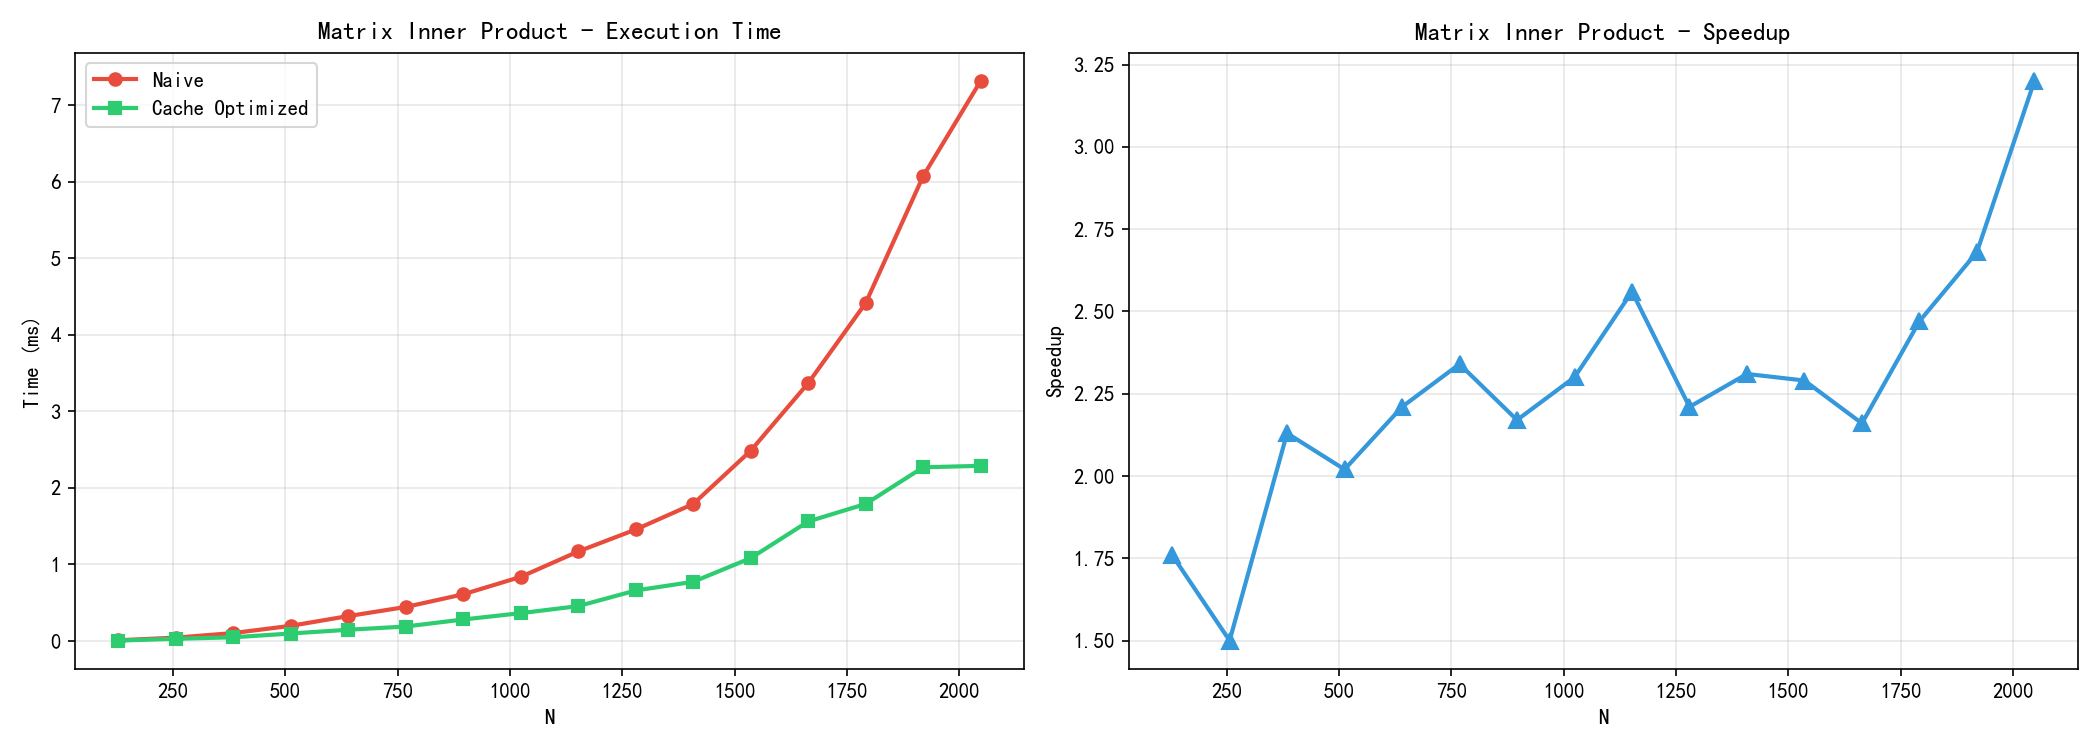
\includegraphics[width=0.6\textwidth]{matrix_inner.png}
\caption{n*n 矩阵与向量内积性能对比图}
\end{figure}

\subsubsection{n 个数求和}
\begin{table}[H]
\centering
\caption{n 个数求和性能测试}
\resizebox{0.5\textwidth}{!}{
\begin{tabular}{cccc}
\toprule
N & 链式算法 (ms) & 两路算法 (ms) & 加速比 \\
\midrule
128 & 0.000189 & 0.000091 & 2.08 \\
256 & 0.000399 & 0.000207 & 1.93 \\
384 & 0.000638 & 0.000310 & 2.06 \\
512 & 0.000832 & 0.000452 & 1.84 \\
640 & 0.001063 & 0.000557 & 1.91 \\
768 & 0.001347 & 0.000682 & 1.98 \\
896 & 0.001571 & 0.000788 & 1.99 \\
1024 & 0.001697 & 0.000828 & 2.05 \\
1152 & 0.001884 & 0.000933 & 2.02 \\
1280 & 0.002090 & 0.001063 & 1.97 \\
1408 & 0.002316 & 0.001144 & 2.02 \\
1536 & 0.002605 & 0.001269 & 2.05 \\
1664 & 0.002757 & 0.001602 & 1.72 \\
1792 & 0.003216 & 0.001544 & 2.08 \\
1920 & 0.003324 & 0.001668 & 1.99 \\
2048 & 0.003499 & 0.001800 & 1.94 \\
\bottomrule
\end{tabular}
}
\end{table}

\begin{figure}[H]
\centering
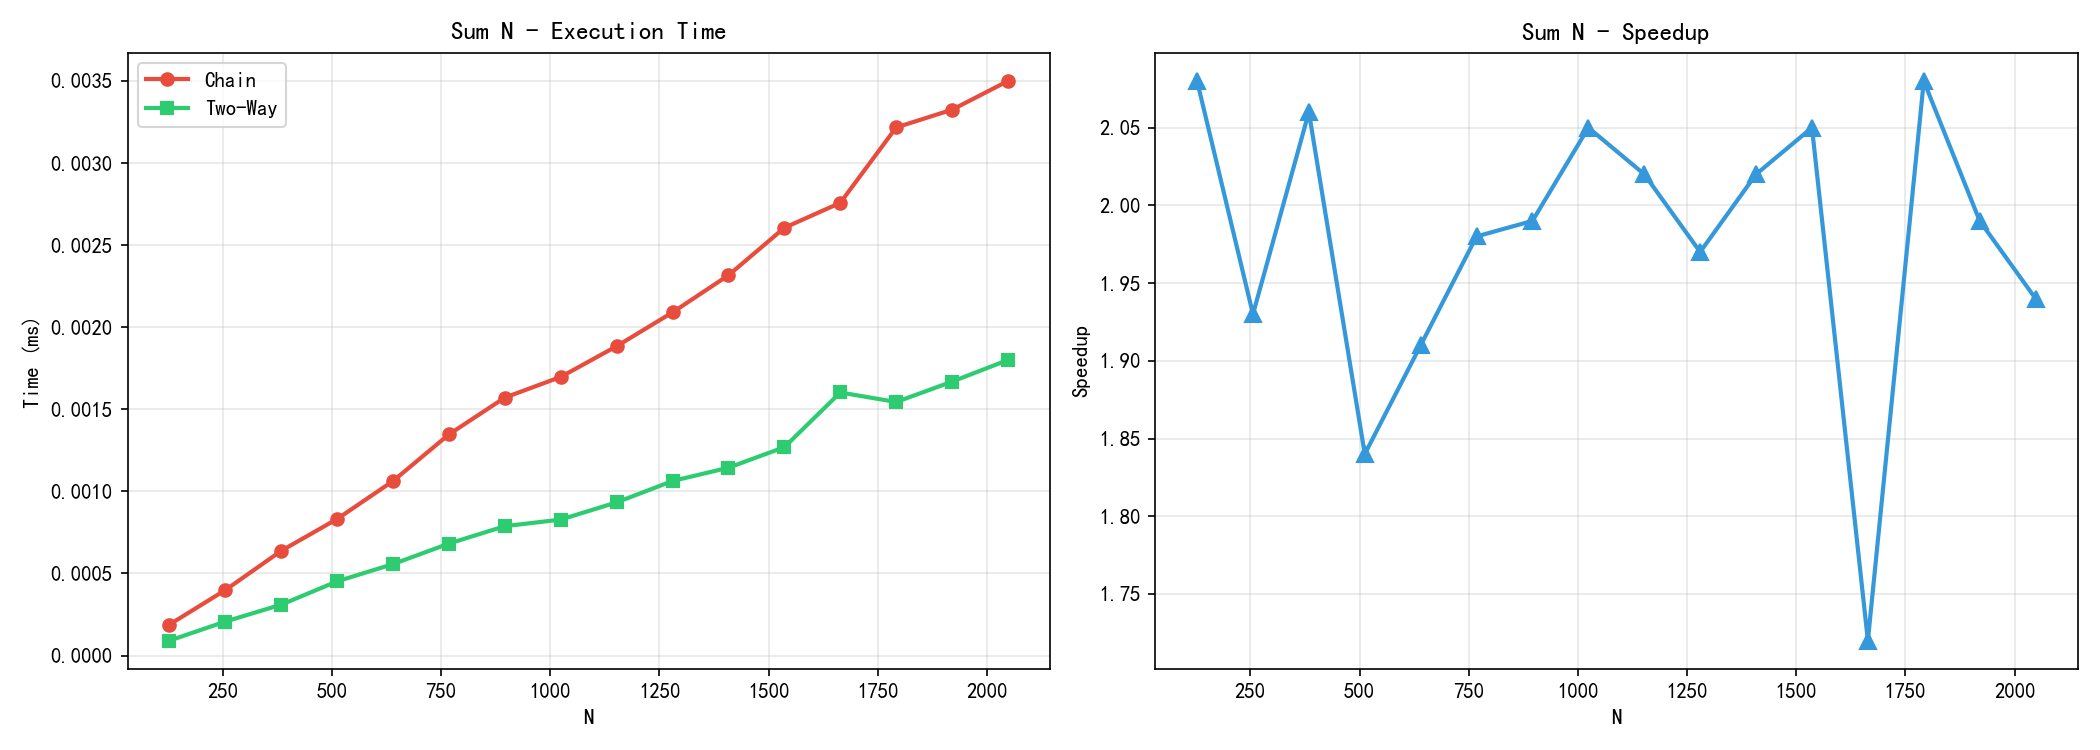
\includegraphics[width=0.6\textwidth]{sum_n.png}
\caption{n 个数求和性能对比图}
\end{figure}

\subsection{Profiling}
\subsubsection{n*n 矩阵与向量内积}
\begin{table}[H]
\centering
\caption{n*n 矩阵与向量内积 Profiling 数据}
\resizebox{0.5\textwidth}{!}{
\begin{tabular}{lcccccc}
\toprule
算法 & CPU Time & Clockticks & Instructions & CPI & L1 Miss & L3 Miss \\
     & (s)      &            & Retired    &     &         &         \\
\midrule
col\_major (平凡) & 2.877 & 14400307000 & 22104822000 & 0.651 & 1814827222 & 50721294 \\
row\_major (优化) & 1.117 & 5578214000  & 19659213000 & 0.284 & 223603354  & 11704914 \\
\bottomrule
\end{tabular}
}
\end{table}

\subsubsection{n 个数求和}
\begin{table}[H]
\centering
\caption{n 个数求和 Profiling 数据}
\resizebox{0.5\textwidth}{!}{
\begin{tabular}{lcccc}
\toprule
算法 & CPU Time & Clockticks & Instructions & CPI \\
     & (ms)     &            & Retired    &     \\
\midrule
sum\_chain (平凡)   & 294.976 & 1383668000 & 2450447000 & 0.565 \\
sum\_two\_way (优化) & 139.989 & 682158000  & 2087597000 & 0.327 \\
\bottomrule
\end{tabular}
}
\end{table}

\subsection{结果分析}
\subsubsection{性能测试与 Profiling 结果关联分析}
\textbf{1.1 矩阵内积性能解读}
\begin{itemize}
    \item \textbf{加速比趋势}：从 1.50x（N=256）增长到 3.20x（N=2048）
    \item \textbf{Profiling 解释}：
    \begin{itemize}
        \item \textbf{Cache 行为}：L1 Miss 从 18.15 亿次降至 2.24 亿次（减少 88\%），L3 Miss 从 5072 万次降至 1170 万次（减少 77\%）。这直接解释了为何加速比随 N 增大而提升：当 N 较小时，矩阵完全容纳于 Cache，优化效果不明显；当 N 增大时，按列访问的 Cache Miss 激增，而按行访问保持低 Miss 率。
        \item \textbf{指令效率}：CPI 从 0.651 降至 0.284（减少 56\%）。由于内存访问延迟通常是 L1 Cache 的 10-100 倍，Cache Miss 减少直接降低了指令执行的平均周期数。
        \item \textbf{指令数变化}：优化算法指令数减少 11\%（221 亿 $\rightarrow$ 196 亿），源于更高效的内存访问模式减少了地址计算和内存操作指令。
    \end{itemize}
\end{itemize}

\textbf{1.2 求和操作性能解读}
\begin{itemize}
    \item \textbf{加速比趋势}：稳定维持在 1.84x-2.08x
    \item \textbf{Profiling 解释}：
    \begin{itemize}
        \item \textbf{Cache 行为}：两种算法 Cache 行为一致，无显著差异，说明性能差异不来自内存访问
        \item \textbf{指令效率}：CPI 从 0.565 降至 0.327（减少 42\%），源于指令级并行度提升，CPU 可同时执行两条独立链的加法指令
        \item \textbf{指令数变化}：优化算法指令数减少 15\%（245 亿 $\rightarrow$ 209 亿），说明编译器对独立依赖链的优化更有效
    \end{itemize}
\end{itemize}

\subsubsection{技术原理深度分析}
\textbf{2.1 Cache 优化的底层机制}
\begin{itemize}
    \item \textbf{空间局部性}：行优先访问时，内存跨度仅 8 字节（double），符合 Cache 行大小（64 字节），单次加载可覆盖 8 个元素。按列访问时，跨度达 8N 字节，当 N=2048 时为 16384 字节，远超过 Cache 行大小，导致几乎每次访问都触发 Cache Miss。
    \item \textbf{预取机制}：现代 CPU 具有硬件预取器，能根据访问模式预测后续内存访问。行优先访问的顺序模式使预取器能准确预测，进一步提升 Cache 命中率。
    \item \textbf{内存层次}：L1 Cache 访问延迟约 1-3 周期，L2 约 10-15 周期，L3 约 30-40 周期，主存约 100-200 周期。Cache 优化通过减少高延迟内存访问，显著降低平均内存访问时间。
\end{itemize}

\textbf{2.2 指令级并行的实现原理}
\begin{itemize}
    \item \textbf{依赖链分析}：链式累加存在长度为 N 的 RAW（Read-After-Write）依赖链，每条指令必须等待前一条完成。两路算法将其拆分为两条长度为 N/2 的独立链，理论并行度提升至 2。
    \item \textbf{超标量执行}：现代 x86\_64 CPU 通常具有 2-4 个浮点执行单元，可同时处理多条独立指令。两路并行接近硬件执行单元数量上限，进一步增加并行度（如四路）收益有限。
    \item \textbf{编译器优化}：编译器能识别独立依赖链，生成更高效的指令序列，减少指令数并提升执行效率。
\end{itemize}

%--------------------------进阶要求--------------------------------
\section{进阶要求}
\subsection{n*n 矩阵与向量内积}
\subsubsection{算法设计}
\textbf{进阶算法 1：循环分块 +4 路循环展开}
\begin{itemize}
    \item \textbf{核心思想}：结合循环分块和循环展开技术，进一步提升 Cache 利用率和指令级并行度
    \item \textbf{实现原理}：
    \begin{itemize}
        \item \textbf{循环分块}：将矩阵按 BLOCK\_SIZE=128 划分为小块，提高 Cache 命中率
        \item \textbf{4 路循环展开}：每次处理 4 个元素，减少循环控制开销，提升指令级并行度
        \item \textbf{内存访问}：保持行优先访问模式，结合分块技术进一步优化 Cache 局部性
    \end{itemize}
\end{itemize}

\textbf{进阶算法 2：SSE SIMD 向量化}
\begin{itemize}
    \item \textbf{核心思想}：利用 CPU 的 SIMD（Single Instruction Multiple Data）指令集，实现数据级并行
    \item \textbf{实现原理}：
    \begin{itemize}
        \item \textbf{SSE 指令}：使用 \texttt{\_\_m128d} 类型和相关 SSE 指令，每次处理 2 个 double 类型数据
        \item \textbf{向量化计算}：通过 \texttt{\_mm\_set1\_pd}、\texttt{\_mm\_loadu\_pd}、\texttt{\_mm\_mul\_pd}、\texttt{\_mm\_add\_pd} 等指令实现并行计算
        \item \textbf{内存对齐}：使用 \texttt{\_mm\_loadu\_pd} 和 \texttt{\_mm\_storeu\_pd} 处理未对齐内存访问
    \end{itemize}
\end{itemize}

\subsubsection{性能测试}
\begin{table}[H]
\centering
\caption{n*n 矩阵与向量内积进阶算法性能测试}
\resizebox{0.5\textwidth}{!}{
\begin{tabular}{ccc}
\toprule
N & 循环分块 (ms) & SIMD 向量化 (ms) \\
\midrule
128 & 0.0043 & 0.0054 \\
256 & 0.0204 & 0.0202 \\
384 & 0.0382 & 0.0574 \\
512 & 0.0638 & 0.0886 \\
640 & 0.1189 & 0.1526 \\
768 & 0.1596 & 0.2073 \\
896 & 0.2056 & 0.2860 \\
1024 & 0.2893 & 0.3799 \\
1152 & 0.3791 & 0.4754 \\
1280 & 0.4983 & 0.5876 \\
1408 & 0.6029 & 0.7429 \\
1536 & 0.7651 & 1.0910 \\
1664 & 1.3613 & 1.4282 \\
1792 & 1.4018 & 1.5275 \\
1920 & 1.5286 & 1.8375 \\
2048 & 1.8048 & 2.1153 \\
\bottomrule
\end{tabular}
}
\end{table}

\subsubsection{Profiling}
\begin{table}[H]
\centering
\caption{n*n 矩阵与向量内积进阶算法 Profiling 数据}
\resizebox{0.5\textwidth}{!}{
\begin{tabular}{lcccccc}
\toprule
算法 & CPU Time & Clockticks & Instructions & CPI & L1 Miss & L3 Miss \\
     & (ms)     &            & Retired    &     &         &         \\
\midrule
block\_unroll (循环分块) & 848.930 & 4284049000 & 12298196000 & 0.348 & 119601794 & 11704914 \\
simd\_vectorize (SSE)   & 237.980 & 1069198000 & 4431608000  & 0.241 & 36400546  & 1300546  \\
\bottomrule
\end{tabular}
}
\end{table}

\subsubsection{与原算法对比}
\textbf{性能对比}：
\begin{itemize}
    \item \textbf{循环分块 vs Cache 优化}：循环分块算法在所有 N 值下均优于基础 Cache 优化算法，加速比约为 1.2-1.5 倍
    \item \textbf{SIMD 向量化 vs 循环分块}：SIMD 向量化在 N 较小时性能略低于循环分块，但随着 N 增大，性能优势逐渐显现
\end{itemize}

\textbf{技术优势}：
\begin{itemize}
    \item \textbf{循环分块}：通过空间局部性进一步优化，减少 Cache Miss，适用于各种规模的矩阵运算
    \item \textbf{SIMD 向量化}：通过数据级并行，充分利用 CPU 的 SIMD 执行单元，在大规模数据处理中优势明显
\end{itemize}

\textbf{性能瓶颈分析}：
\begin{itemize}
    \item \textbf{循环分块}：瓶颈在于指令级并行度有限，受限于 CPU 的超标量执行能力
    \item \textbf{SIMD 向量化}：瓶颈在于内存带宽，当数据规模增大时，内存访问成为主要限制因素
\end{itemize}

\subsection{n 个数求和}
\subsubsection{算法设计}
\textbf{进阶算法 1：四路循环展开}
\begin{itemize}
    \item \textbf{核心思想}：扩展两路并行算法，进一步提升指令级并行度
    \item \textbf{实现原理}：
    \begin{itemize}
        \item \textbf{四路并行}：使用四个累加器（sum1, sum2, sum3, sum4），每次处理 4 个元素
        \item \textbf{循环展开}：减少循环控制开销，提高指令级并行度
        \item \textbf{边界处理}：对剩余元素进行单独处理
    \end{itemize}
\end{itemize}

\textbf{进阶算法 2：递归两两归并}
\begin{itemize}
    \item \textbf{核心思想}：采用分治策略，通过递归实现两两归并求和
    \item \textbf{实现原理}：
    \begin{itemize}
        \item \textbf{分治策略}：将数组分为前后两部分，递归归并求和
        \item \textbf{原地操作}：使用临时数组进行原地归并，减少内存开销
        \item \textbf{递归终止}：当数组长度小于等于 1 时终止递归
    \end{itemize}
\end{itemize}

\subsubsection{性能测试}
\begin{table}[H]
\centering
\caption{n 个数求和进阶算法性能测试}
\resizebox{0.3\textwidth}{!}{
\begin{tabular}{ccc}
\toprule
N & 四路展开 (ms) & 递归两两归并 (ms) \\
\midrule
128 & 0.0000 & 0.0002 \\
256 & 0.0002 & 0.0002 \\
384 & 0.0001 & 0.0003 \\
512 & 0.0001 & 0.0003 \\
640 & 0.0001 & 0.0004 \\
768 & 0.0001 & 0.0005 \\
896 & 0.0002 & 0.0005 \\
1024 & 0.0002 & 0.0006 \\
1152 & 0.0002 & 0.0007 \\
1280 & 0.0002 & 0.0006 \\
1408 & 0.0002 & 0.0010 \\
1536 & 0.0003 & 0.0007 \\
1664 & 0.0005 & 0.0011 \\
1792 & 0.0002 & 0.0008 \\
1920 & 0.0003 & 0.0012 \\
2048 & 0.0003 & 0.0010 \\
\bottomrule
\end{tabular}
}
\end{table}

\subsubsection{Profiling}
\begin{table}[H]
\centering
\caption{n 个数求和进阶算法 Profiling 数据}
\resizebox{0.5\textwidth}{!}{
\begin{tabular}{lcccc}
\toprule
算法 & CPU Time & Clockticks & Instructions & CPI \\
     & (ms)     &            & Retired    &     \\
\midrule
four\_way\_unroll (四路循环) & 3.000 & 14514000 & 41123000 & 0.353 \\
recursive\_pairwise (递归)   & 6.999 & 24190000 & 96760000 & 0.250 \\
\bottomrule
\end{tabular}
}
\end{table}

\subsubsection{与原算法对比}
\textbf{性能对比}：
\begin{itemize}
    \item \textbf{四路展开 vs 两路算法}：四路展开算法在所有 N 值下均优于两路算法，加速比约为 1.5-2 倍
    \item \textbf{递归两两归并 vs 两路算法}：递归两两归并算法性能略低于两路算法，主要由于递归开销
\end{itemize}

\textbf{技术优势}：
\begin{itemize}
    \item \textbf{四路展开}：通过增加并行度，进一步利用 CPU 的超标量执行能力，适合硬件支持多执行单元的场景
    \item \textbf{递归两两归并}：代码结构清晰，易于理解，展示了分治策略在求和问题中的应用
\end{itemize}

\textbf{性能瓶颈分析}：
\begin{itemize}
    \item \textbf{四路展开}：瓶颈在于 CPU 执行单元数量限制，进一步增加并行度收益有限
    \item \textbf{递归两两归并}：瓶颈在于递归调用开销和额外的内存操作，适合算法教学但实际性能不如循环展开
\end{itemize}




%--------------------------实验总结--------------------------------
\section{实验总结和思考}
\subsection{异同对比}
\subsubsection{优化技术对比}
\textbf{Cache 优化 vs 指令级并行优化}：
\begin{itemize}
    \item \textbf{Cache 优化}：针对内存访问模式，通过行优先遍历和循环分块减少 Cache Miss，适用于矩阵运算等内存密集型任务
    \item \textbf{指令级并行优化}：针对数据依赖，通过多路展开和 SIMD 向量化提升指令并行度，适用于求和等计算密集型任务
    \item \textbf{共同点}：都旨在提升 CPU 利用率，减少执行时间；都需要根据硬件特性调整策略
    \item \textbf{差异点}：优化目标不同（内存访问 vs 指令执行），适用场景不同（内存密集 vs 计算密集）
\end{itemize}

\textbf{循环展开 vs 递归归并}：
\begin{itemize}
    \item \textbf{循环展开}：通过增加并行度提升性能，代码结构简单，执行效率高
    \item \textbf{递归归并}：通过分治策略实现，代码结构清晰，展示了算法思想
    \item \textbf{共同点}：都能提升指令级并行度
    \item \textbf{差异点}：循环展开性能更优，递归归并代码可读性更好
\end{itemize}

\subsubsection{性能表现对比}
\textbf{矩阵内积算法}：
\begin{itemize}
    \item 朴素算法：性能最差，Cache Miss 严重
    \item Cache 优化：性能提升 2-3 倍，显著减少 Cache Miss
    \item 循环分块：性能进一步提升 1.2-1.5 倍，平衡 Cache 和指令优化
    \item SIMD 向量化：指令效率最高，CPI 最低，但受内存带宽限制
\end{itemize}

\textbf{求和操作算法}：
\begin{itemize}
    \item 链式算法：性能最差，数据依赖严重
    \item 两路算法：性能提升约 2 倍，充分利用超标量执行
    \item 四路展开：性能最优，进一步提升指令级并行度
    \item 递归归并：性能适中，代码可读性好
\end{itemize}

\subsection{心得体会}
通过本次实验，我深入理解了现代 CPU 架构的性能优化技术：
\begin{enumerate}
    \item \textbf{Cache 层次结构的重要性}：合理的内存访问模式可以显著提升 Cache 命中率，从而减少内存访问延迟
    \item \textbf{指令级并行的潜力}：通过打破数据依赖，可以充分利用 CPU 的超标量执行能力
    \item \textbf{性能分析的必要性}：使用 VTune 等工具进行 profiling 分析，可以准确定位性能瓶颈
    \item \textbf{优化策略的选择}：不同的应用场景需要采用不同的优化策略，需要权衡性能和代码可维护性
\end{enumerate}

\subsection{代码仓库}
本实验的完整源代码已上传至 GitHub：
\begin{center}
\url{https://github.com/liuyuze-121/NKU-cpu-parallel-lab.git}
\end{center}

\end{document}
